\documentclass[aspectratio=169,10pt]{beamer}

\usepackage{amsmath, amssymb, amsfonts}
\usepackage{xcolor}
\usepackage{listings}
\usepackage{graphicx}
\usepackage{xfrac}
\usepackage{array}

\usetheme{Madrid}
\usecolortheme{seahorse}

\graphicspath{{figures/}}

\lstset{
    basicstyle=\ttfamily\scriptsize,
    keywordstyle=\color{blue},
    commentstyle=\color{green!50!black}\itshape,
    stringstyle=\color{red},
    numbers=left,
    numberstyle=\tiny\color{gray},
    frame=single,
    breaklines=true,
    language=Python,
    showspaces=false,
    showtabs=false,
    tabsize=2
}

\setbeamertemplate{footline}[frame number]

% Title Page
\title[Ch. 29: Projection Operators]{Chapter 29: Projection Operators}
\subtitle{Convex Analysis and Monotone Operator Theory}
\author{Based on Bauschke \& Combettes (2017)}
\date{Pages 951--990}

\begin{document}

\begin{frame}
    \titlepage
\end{frame}

% Outline
\begin{frame}{Outline}
    \tableofcontents
\end{frame}

% ============================================================================
% SECTION 1: INTRODUCTION
% ============================================================================
\section{Introduction \& Motivation}

\begin{frame}[fragile]{What Are Projection Operators?}
    \begin{itemize}
        \item \textbf{Definition}: For a nonempty closed convex set $C \subseteq \mathcal{H}$, the \textit{projection} of $x \in \mathcal{H}$ onto $C$ is:
        $$P_C(x) = \arg\min_{y \in C} \|x - y\|$$

        \item \textbf{Key Properties}:
        \begin{enumerate}
            \item Uniqueness: The minimizer is unique for convex sets
            \item Characterization: $P_C(x) \in C$ and $\langle x - P_C(x) \mid y - P_C(x) \rangle \leq 0$ for all $y \in C$
            \item Nonexpansiveness: $\|P_C(x) - P_C(y)\| \leq \|x - y\|$
        \end{enumerate}

        \item \textbf{Applications}:
        \begin{enumerate}
            \item Convex optimization via projection algorithms
            \item Constraint satisfaction in feasibility problems
            \item Signal processing and image reconstruction
            \item Machine learning (proximal methods)
        \end{enumerate}
    \end{itemize}
\end{frame}

\begin{frame}{Geometric Intuition}
    \begin{columns}
        \column{0.5\textwidth}
        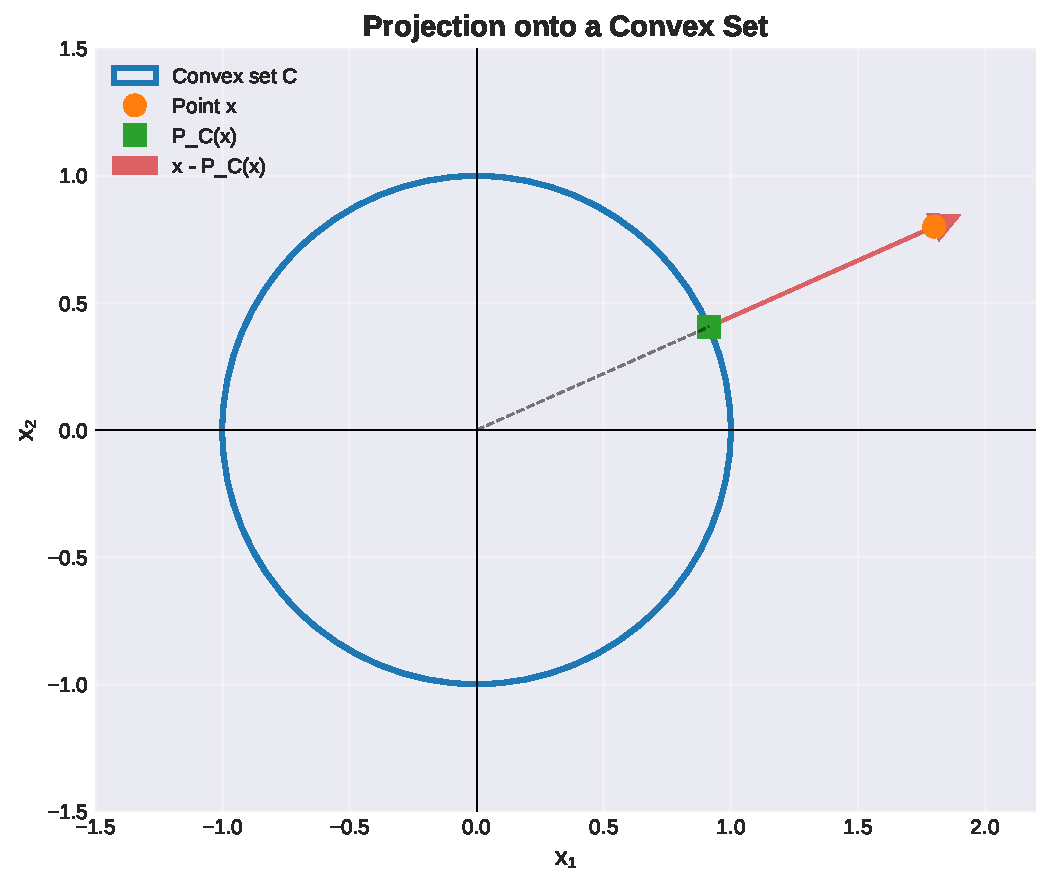
\includegraphics[width=\textwidth]{fig_projection_concept.pdf}

        \column{0.5\textwidth}
        \begin{itemize}
            \item The projection $P_C(x)$ is the point in $C$ \textbf{closest} to $x$

            \item The residual vector $x - P_C(x)$ is \textbf{orthogonal} to $C$ at $P_C(x)$

            \item This is the \textit{normal cone} property

            \item Generalizes familiar concept: projection onto a line or plane
        \end{itemize}
    \end{columns}
\end{frame}

% ============================================================================
% SECTION 2: BASIC PROPERTIES
% ============================================================================
\section{Basic Properties (Section 29.1)}

\begin{frame}[allowframebreaks]{Key Propositions: Part I}

    \textbf{Proposition 29.1} (Existence and Uniqueness):\\
    For $K$ nonempty closed convex subset of $\mathcal{H}$ and $L \in \mathcal{B}(\mathcal{H}, \mathcal{K})$, if $C = \mathcal{R}(L)$ is the range, then:
    \begin{align*}
    P_C x = x + L^*(\gamma \text{Id} - L L^*)^{-1}(Lx)
    \end{align*}
    for suitable $\gamma > 0$.

    \vspace{0.5cm}

    \textbf{Proposition 29.2} (Scaled Operators):\\
    For invertible $L$:
    $$P_D x = L^{-1} P_C(Lx)$$
    where $D = L^{-1}(C)$.

    \vspace{0.5cm}

    \textbf{Proposition 29.3} (Product Spaces):\\
    For finite family $(H_i)_{i \in I}$ and closed convex sets $C_i \subseteq H_i$:
    $$P_{\bigoplus_i C_i} x = (P_{C_i} x_i)_{i \in I}$$

    \framebreak

    \textbf{Proposition 29.5} (Nested Projections):\\
    If $P_C x \in D$ for nonempty closed convex sets $C, D$:
    $$P_{C \cap D} x = P_C x$$

    \vspace{0.5cm}

    \textbf{Proposition 29.6} (Direct Sum Decomposition):\\
    For $C \perp D$ (orthogonal decomposition):
    $$P_{C+D} = P_C + P_D$$

    \vspace{0.5cm}

    \textbf{Proposition 29.7 \& 29.8}:\\
    Monotonic sequences of sets preserve properties:
    \begin{itemize}
        \item If $C_n \subseteq C_{n+1}$ and $C = \bigcup_n C_n$, then $P_C x \leftarrow P_{C_n} x$
        \item If $C_n \supseteq C_{n+1}$ with $\bigcap_n C_n \neq \emptyset$, then $P_C x \leftarrow P_{C_n} x$
    \end{itemize}

\end{frame}

\begin{frame}{Characterization via Variational Inequality}

    \textbf{Core Property} (Equation 29.1):\\
    The projection $P_C(x)$ is characterized by:
    $$\forall y \in C: \quad \langle x - P_C(x) \mid y - P_C(x) \rangle \leq 0$$

    \vspace{0.5cm}

    \textit{Interpretation}: The residual vector $x - P_C(x)$ makes an \textbf{obtuse angle} with any direction $y - P_C(x)$ pointing into $C$.

    \vspace{0.5cm}

    \textbf{Equivalence}: This is equivalent to saying $x - P_C(x) \in N_C(P_C(x))$, where $N_C$ is the \textit{normal cone} to $C$ at $P_C(x)$.

    \vspace{0.5cm}

    \textbf{Lemma 29.12}:\\
    For $\alpha, \beta \in \mathbb{R}_{++}$ with $\alpha < \beta$ and $D = -\gamma + C$ where $\gamma = \beta/\alpha$:
    $$\phi(\beta) = \beta^{-1}\|P_D(\beta x)\|$$
    is decreasing in $\beta$.

\end{frame}

\begin{frame}{Nonexpansiveness and Firm Nonexpansiveness}

    \textbf{Corollary 29.12} (Key Inequality):\\
    Define $\phi(\alpha) = \alpha^{-1}\|P_C(\alpha x) - y\|$ for $0 < \alpha < \beta$ and any $y \in \mathcal{H}$.\\
    Then $\phi$ is \textbf{decreasing in $\alpha$}.

    \vspace{0.5cm}

    \textbf{Proposition 29.11} (Lipschitz Continuity):\\
    For $C$ nonempty closed convex and $\gamma \in ]1, +\infty[$:
    $$\|P_C(\gamma x)\| \leq \gamma \|P_C x\|$$

    \vspace{0.5cm}

    \textbf{Firm Nonexpansiveness}:\\
    The projection operator satisfies:
    \begin{align*}
    \|P_C x - P_C y\|^2 \leq \langle x - y \mid P_C x - P_C y \rangle
    \end{align*}

    This is \textit{stronger} than ordinary nonexpansiveness!

\end{frame}

\begin{frame}{Visualizing Nonexpansiveness}
    \begin{columns}
        \column{0.5\textwidth}
        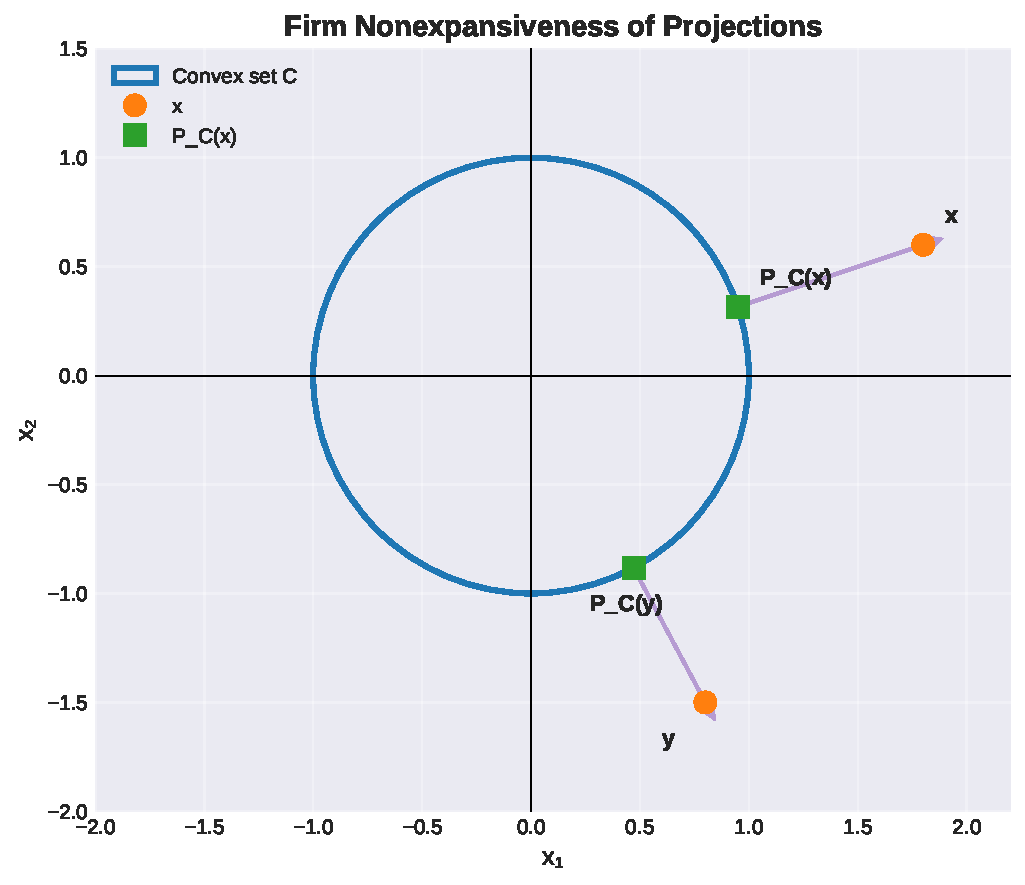
\includegraphics[width=\textwidth]{fig_nonexpansiveness.pdf}

        \column{0.5\textwidth}
        \begin{itemize}
            \item Projection operators \textit{contract} distances between points

            \item The contraction is \textit{firm}: stronger than simple nonexpansiveness

            \item Distance between projections $\leq$ distance between original points

            \item This property is \textbf{critical} for convergence analysis
        \end{itemize}
    \end{columns}
\end{frame}

% ============================================================================
% SECTION 3: AFFINE SUBSPACES
% ============================================================================
\section{Affine Subspaces (Section 29.2)}

\begin{frame}[allowframebreaks]{Projections onto Affine Subspaces}

    \textbf{Proposition 29.14}:\\
    For closed affine subspace $C$ and $x, y \in \mathcal{H}$, $z \in C$:
    \begin{enumerate}
        \item[(i)] $P_C$ is weakly continuous
        \item[(ii)] $x - P_C x \perp C - C$ (orthogonal to direction space)
        \item[(iii)] $\|x - P_C y\|^2 = \|P_C x - P_C y\|^2 + \|({\rm Id} - P_C)x - ({\rm Id} - P_C)y\|^2$
        \item[(iv)] $\|(2P_C - {\rm Id})x - (2P_C - {\rm Id})y\| = \|x - y\|$ (reflection)
        \item[(v)] $\|P_C x - P_C y\|^2 = \langle x - y \mid P_C x - P_C y \rangle$
        \item[(vi)] $\|({\rm Id} - P_C)x - ({\rm Id} - P_C)y\|^2 = \langle x - y \mid ({\rm Id} - P_C)x - ({\rm Id} - P_C)y \rangle$
        \item[(vii)] $\|x - P_C x\|^2 = \langle x - z \mid x - P_C x \rangle$
    \end{enumerate}

    \framebreak

    \textbf{Proposition 29.15} (Orthonormal Basis):\\
    If $(e_i)_{i \in I}$ is orthonormal with $C = \overline{\text{span}} \{e_i\}$:
    $$P_C x = \sum_{i \in I} \langle x \mid e_i \rangle e_i$$

    \textit{Example}: Projection onto line $U = \mathbb{R} u$ with $\|u\| = 1$:
    $$P_U x = \langle x \mid u \rangle u$$

    \vspace{0.5cm}

    \textbf{Proposition 29.16}:\\
    For weighted Hilbert space with weights $(w_i)_{i \in I}$:
    $$\langle x, y \rangle = \sum_{i \in I} w_i \langle x_i \mid y_i \rangle$$
    The projection onto $D = \{(x)_{i \in I} : x \in \mathcal{H}\}$ is:
    $$P_D x = (p)_{i \in I} \text{ where } p = \sum_{i \in I} w_i x_i$$

\end{frame}

\begin{frame}{Geometric Illustration}
    \begin{columns}
        \column{0.5\textwidth}
        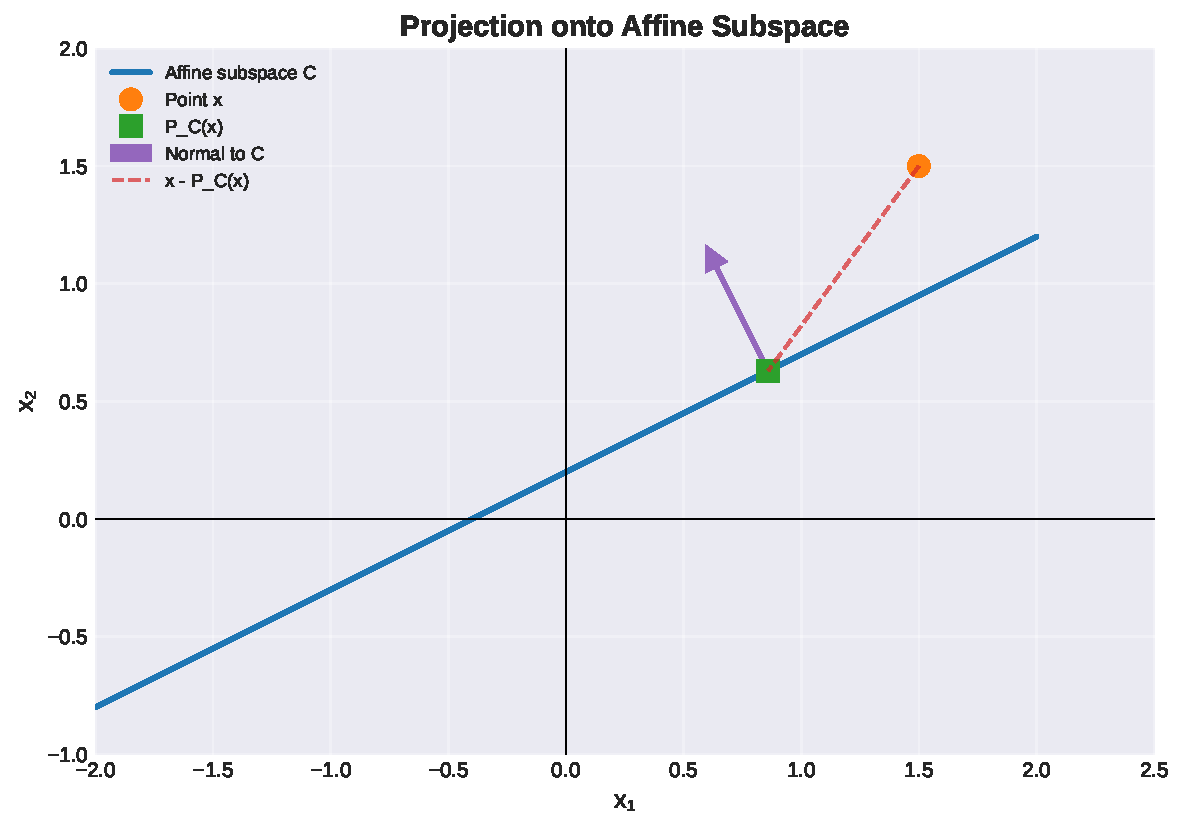
\includegraphics[width=\textwidth]{fig_projection_affine.pdf}

        \column{0.5\textwidth}
        \begin{itemize}
            \item Affine subspaces are \textbf{translates} of linear subspaces

            \item Projection is \textbf{orthogonal} to the subspace direction

            \item For orthonormal bases, projection is \textbf{simply} the sum of coordinate components

            \item Used extensively in least-squares problems
        \end{itemize}
    \end{columns}
\end{frame}

% ============================================================================
% SECTION 4: SPECIAL POLYHEDRA
% ============================================================================
\section{Projections onto Special Polyhedra (Sect. 29.3--29.4)}

\begin{frame}[allowframebreaks]{Projections onto Half-Spaces}

    \textbf{Example 29.20} (Half-Space):\\
    For $u \in \mathcal{H} \setminus \{0\}$ and $\eta \in \mathbb{R}$, the half-space:
    $$C = \{x \in \mathcal{H} : \langle x \mid u \rangle \leq \eta\}$$

    Exactly one of the following holds:

    \begin{enumerate}
        \item[(i)] $u = 0$ and $\eta \geq 0$: then $C = \mathcal{H}$ and $P_C = {\rm Id}$
        \item[(ii)] $u = 0$ and $\eta < 0$: then $C = \emptyset$
        \item[(iii)] $u \neq 0$:
        $$P_C x = \begin{cases}
        x & \text{if } \langle x \mid u \rangle \leq \eta \\
        x + \frac{\eta - \langle x \mid u \rangle}{\|u\|^2} u & \text{if } \langle x \mid u \rangle > \eta
        \end{cases}$$
    \end{enumerate}

    \framebreak

    \textbf{Example 29.21} (Slab):\\
    For $\eta_1 \leq \eta_2$ and nonzero $u$:
    $$C = \{x \in \mathcal{H} : \eta_1 \leq \langle x \mid u \rangle \leq \eta_2\}$$

    With $\phi: t \mapsto \sum_{i \in I} \max\{\xi_i, t, 0\}$, the projection is:
    $$P_C x = \begin{cases}
    x + \frac{\eta_1 - \langle x \mid u \rangle}{\|u\|^2} u & \text{if } \langle x \mid u \rangle < \eta_1 \\
    x & \text{if } \eta_1 \leq \langle x \mid u \rangle \leq \eta_2 \\
    x + \frac{\eta_2 - \langle x \mid u \rangle}{\|u\|^2} u & \text{if } \langle x \mid u \rangle > \eta_2
    \end{cases}$$

    \vspace{0.3cm}

    \framebreak

    \textbf{Proposition 29.22} (Two Parallel Half-Spaces):\\
    For linearly independent $u_1, u_2$ with $\eta_1, \eta_2 \in \mathbb{R}$:
    $$C = \{x : \langle x \mid u_1 \rangle \leq \eta_1\} \cap \{x : \langle x \mid u_2 \rangle \leq \eta_2\}$$

    Closed-form expressions for $P_C x$ in terms of:
    \begin{align*}
    \nu_1 = \frac{\|u_2\|^2(\langle x \mid u_1 \rangle - \eta_1) - \langle u_1 \mid u_2 \rangle(\langle x \mid u_2 \rangle - \eta_2)}{\|u_1\|^2\|u_2\|^2 - \langle u_1 \mid u_2 \rangle^2}
    \end{align*}

\end{frame}

\begin{frame}{Half-Space Projection Example}
    \begin{columns}
        \column{0.5\textwidth}
        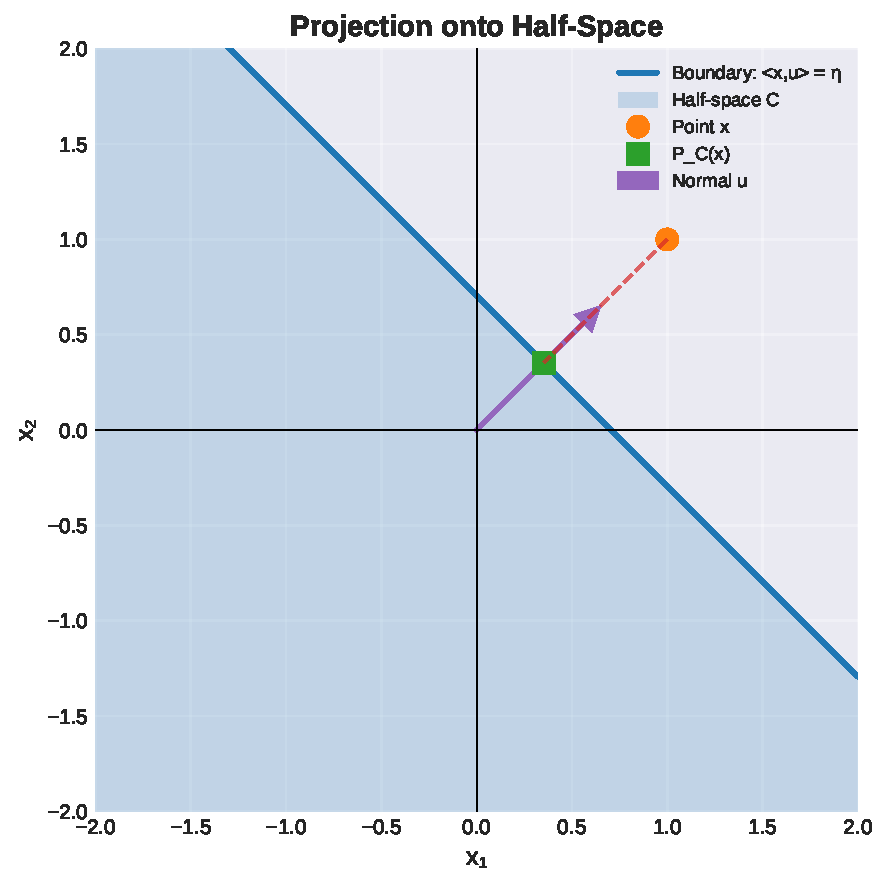
\includegraphics[width=\textwidth]{fig_projection_halfspace.pdf}

        \column{0.5\textwidth}
        \begin{itemize}
            \item Simplest nontrivial case: \textit{half-space}

            \item Projection direction is \textbf{normal} to the boundary

            \item If $x$ already satisfies constraint, no movement

            \item Otherwise, move along normal by amount:
            $$\frac{\eta - \langle x \mid u \rangle}{\|u\|^2}$$
        \end{itemize}
    \end{columns}
\end{frame}

\begin{frame}[allowframebreaks]{Projections onto Simplices}

    \textbf{Proposition 29.26} (Projection onto Convex Hull):\\
    For finite set $\{x_1, \ldots, x_m\}$ and $C = \text{conv}\{x_i\}_{i \in I}$:
    $$P_C x = \sum_{i \in I} \bar{\alpha}_i x_i$$
    where $(\bar{\alpha}_i)$ solves:
    \begin{align*}
    \min_{\alpha \in \mathbb{R}_+^m, \sum \alpha_i = 1} \sum_{i,j} \alpha_i\alpha_j \langle x_i \mid x_j \rangle - 2\sum_i \alpha_i \langle x_i \mid x \rangle
    \end{align*}

    \vspace{0.3cm}

    \textbf{Example 29.27} (Probability Simplex):\\
    For $\mathcal{H} = \mathbb{R}^N$ and:
    $$\Delta = \{x \in \mathbb{R}_+^N : \sum_i x_i = 1\}$$

    The projection $P_\Delta$ can be computed via:
    $$P_\Delta = {\rm Id} - \text{Prox}_f$$
    where $f$ is determined by the simplex structure.

    \vspace{0.3cm}

    \framebreak

    \textbf{Example 29.28} ($\ell^1$ Unit Ball):\\
    For $C = \{x \in \mathcal{H} : \|x\|_1 \leq 1\}$:
    $$P_C x = (\text{sign}(\xi_i) \pi_i)_{i \in I}$$
    where $\pi = P_\Delta(|\xi|)$ and $\Delta$ is the probability simplex.

    \vspace{0.3cm}

    Uses coordinate-wise thresholding combined with probability simplex projection.

\end{frame}

\begin{frame}{Simplex Projection Visualization}
    \begin{columns}
        \column{0.5\textwidth}
        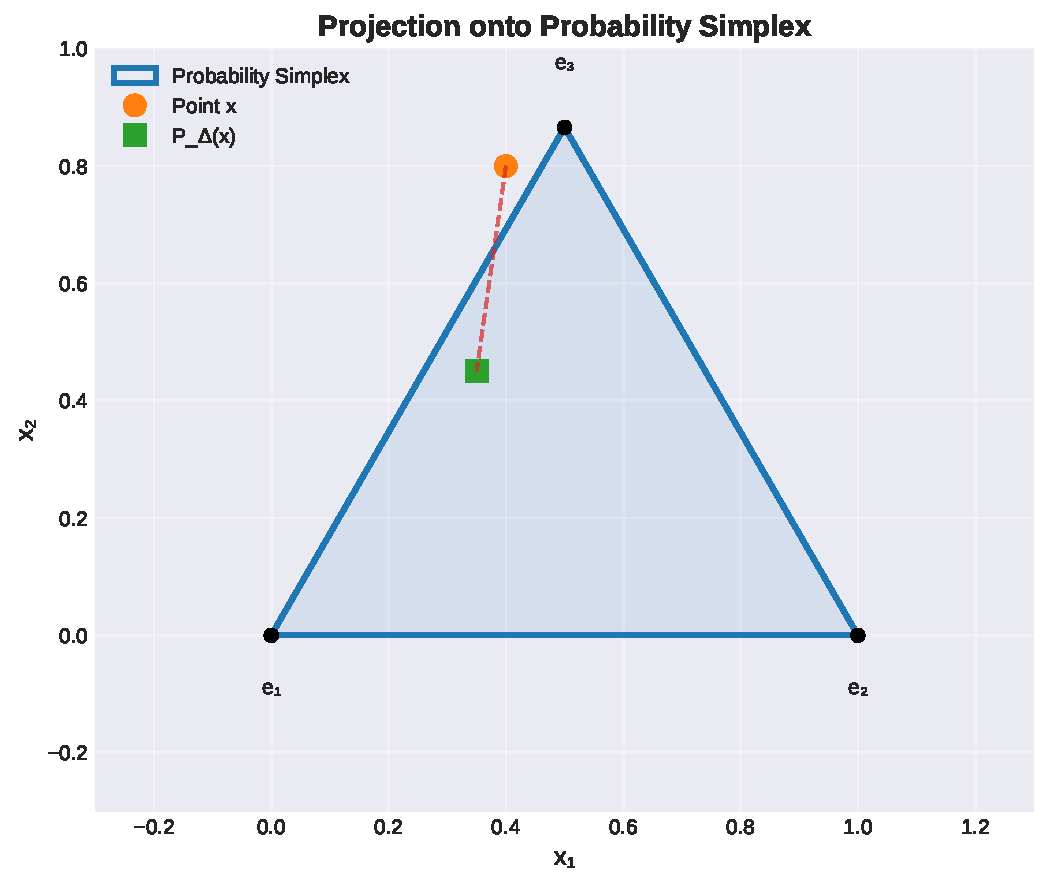
\includegraphics[width=\textwidth]{fig_projection_simplex.pdf}

        \column{0.5\textwidth}
        \begin{itemize}
            \item \textbf{Probability simplex}: points with non-negative coordinates summing to 1

            \item \textbf{Important in}: machine learning, statistics, economics

            \item Projection can be solved \textit{efficiently} using sorting

            \item Soft-thresholding operations are key ingredient

            \item Example: sparse recovery, compressed sensing
        \end{itemize}
    \end{columns}
\end{frame}

\begin{frame}{Box Constraint Projection}
    \begin{columns}
        \column{0.5\textwidth}
        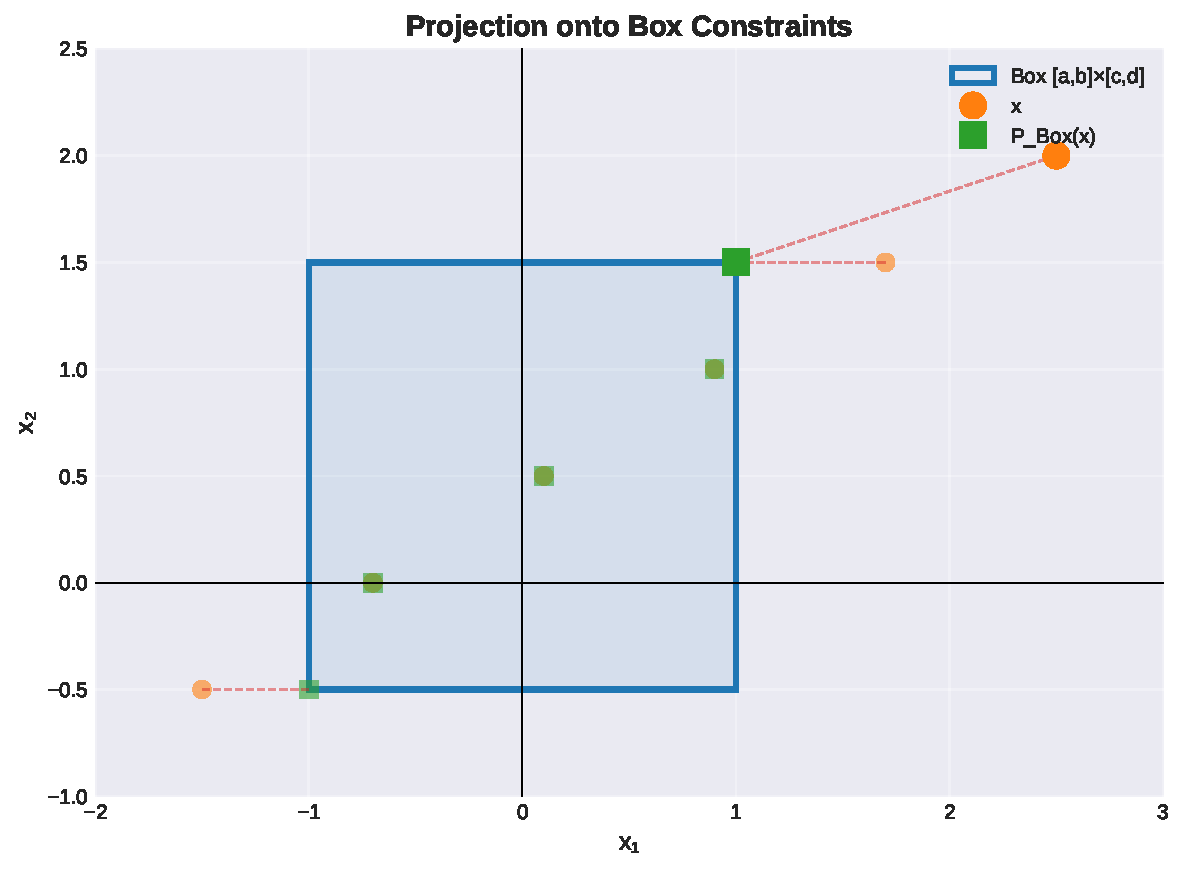
\includegraphics[width=\textwidth]{fig_projection_box.pdf}

        \column{0.5\textwidth}
        \begin{itemize}
            \item \textbf{Box constraints}: $C = [a,b] \times [c,d] \times \cdots$

            \item \textbf{Element-wise clipping}:
            $$P_C(x) = (\text{clip}(x_1, a, b), \text{clip}(x_2, c, d), \ldots)$$
            where $\text{clip}(\xi, a, b) = \max(a, \min(\xi, b))$

            \item \textbf{Complexity}: $O(n)$ for $n$ dimensions

            \item \textbf{Application}: bounded optimization, imaging
        \end{itemize}
    \end{columns}
\end{frame}

% ============================================================================
% SECTION 5: EPIGRAPHS AND LEVEL SETS
% ============================================================================
\section{Epigraphs and Level Sets (Section 29.5)}

\begin{frame}[allowframebreaks]{Projections onto Epigraphs}

    \textbf{Proposition 29.35}:\\
    Let $f: \mathcal{H} \to \mathbb{R}$ be convex continuous, $C = \text{epi } f$, and $(z, \zeta) \in \mathcal{H} \times \mathbb{R}$.\\
    Then the inclusion $z \in x + (f(x) - \zeta)\partial f(x)$ has unique solution $\bar{x}$, and:
    $$P_C(z, \zeta) = (\bar{x}, f(\bar{x}))$$

    \vspace{0.5cm}

    \textbf{Example 29.36}:\\
    For quadratic $f(x) = \frac{1}{2}\sum_i \alpha_i \xi_i^2$, projection yields:
    $$\bar{\xi}_i = \frac{\zeta_i}{(\eta - \zeta)\alpha_i + 1}$$
    where $\eta = f(\bar{x})$ solves the one-dimensional equation.

    \framebreak

    \textbf{Proposition 29.37}:\\
    For $f \in \Gamma_0(\mathcal{H})$ with $\zeta \in \text{int } f(\mathcal{H}), f(\zeta)$ and $C \subseteq \text{dom } f$:

    The equation $f(\text{Prox}_{\partial f} z) = \zeta$ has at least one solution.\\
    If $\bar{\nu}$ is a solution, then:
    $$P_C z = \text{Prox}_{\partial f} \bar{\nu} z$$

\end{frame}

\begin{frame}{Projections onto Lower Level Sets}

    \textbf{Proposition 29.35 (Continued)}:\\
    For epigraph $C = \text{epi } f$ where $f$ is convex continuous:

    The inclusion $z \in x + (f(x) - \zeta)\partial f(x)$ provides the projection characterization.

    \vspace{0.5cm}

    \textbf{Key Insight}:\\
    Projection onto level sets $\text{lev}_{\leq \zeta} f = \{x : f(x) \leq \zeta\}$ reduces to:
    \begin{enumerate}
        \item If $f(x) \leq \zeta$: $P_C x = x$ (already feasible)
        \item If $f(x) > \zeta$: Move along subdifferential direction $\partial f(x)$ until reaching level $\zeta$
    \end{enumerate}

    \vspace{0.5cm}

    \textbf{Application}:\\
    Critical for \textit{level set projection algorithms} used in constrained optimization.

\end{frame}

% ============================================================================
% SECTION 6: ALGORITHMS
% ============================================================================
\section{Subgradient Projection Algorithms (Section 29.6)}

\begin{frame}[allowframebreaks]{Subgradient Projector and Fixed Points}

    \textbf{Motivation}:\\
    For projection operator onto epi-graph, define:
    $$G x = \begin{cases}
    P_C(x + \alpha_n \frac{\mu - f(x_n)}{s(x_n)} s(x_n)) & \text{if } s(x_n) \neq 0 \\
    x_n & \text{if } s(x_n) = 0
    \end{cases}$$
    where $s$ is a selection of $\partial f$.

    \vspace{0.5cm}

    \textbf{Key Examples}:\\

    \textbf{Example 29.47}:\\
    For $f: \mathbb{R} \to \mathbb{R}$, $f(x) = \max\{x+1, 2x+1\}$:
    $$G x = \begin{cases}
    x & \text{if } x \leq -1 \\
    -1 & \text{if } -1 < x < 0 \\
    [-1/2, -1/2] & \text{if } x = 0 \\
    -1/2 & \text{if } x > 0
    \end{cases}$$

    So $G$ is \textbf{discontinuous} despite $f$ being smooth everywhere!

    \framebreak

    \textbf{Example 29.48}\\
    For $\mathcal{H} = \ell^2(\mathbb{N} \setminus \{0\})$ with:
    $$f: (\zeta_n) \mapsto \sum_{n \in \mathbb{N}} n\zeta_n^{2n}$$

    The subgradient projector:
    - Is \textbf{not weakly continuous}
    - Is \textbf{not nonexpansive}
    - Despite $f$ being convex and continuous

    \vspace{0.5cm}

    These examples show limitations of subgradient approaches!

\end{frame}

\begin{frame}[allowframebreaks]{Polyak's Subgradient Projection Algorithm}

    \textbf{Corollary 29.50} (Polyak's Algorithm):\\
    Let $C$ be closed convex, $f: \mathcal{H} \to \mathbb{R}$ continuous convex with $\text{Argmin}_C f \neq \emptyset$.\\
    Suppose one of:
    \begin{enumerate}
        \item[(i)] $f$ bounded on every bounded subset
        \item[(ii)] $f^*$ supercoercive
        \item[(iii)] $\mathcal{H}$ finite-dimensional
    \end{enumerate}

    Let $(\alpha_n)_{n \in \mathbb{N}}$ be sequence with $0 < \inf_n \alpha_n \leq \sup_n \alpha_n < 2$, $s$ a selection of $\partial f$, $x_0 \in C$, $\mu = \min f(C)$:

    \vspace{0.3cm}

    \textbf{Algorithm}:
    $$x_{n+1} = \begin{cases}
    P_C\left(x_n + \alpha_n \frac{\mu - f(x_n)}{s(x_n)^2} s(x_n)\right) & \text{if } s(x_n) \neq 0 \\
    x_n & \text{if } s(x_n) = 0
    \end{cases}$$

    \vspace{0.3cm}

    \framebreak

    \textbf{Convergence Result}:\\
    Then $(x_n)_{n \in \mathbb{N}}$ converges weakly to a minimizer of $f$ over $C$.

    \vspace{0.5cm}

    \textbf{Key Advantages}:
    \begin{enumerate}
        \item Works with \textit{only} subgradients (not full derivatives)
        \item Handles non-smooth objectives
        \item Step size $\mu - f(x_n)$ is \textit{adaptive}
        \item Natural normalization by $\|s(x_n)\|^2$
    \end{enumerate}

    \vspace{0.5cm}

    \textbf{Key Limitations}:
    \begin{enumerate}
        \item Requires knowledge of minimum value $\mu$
        \item Weak convergence only (not strong)
        \item Slow for ill-conditioned problems
    \end{enumerate}

\end{frame}

\begin{frame}{Algorithm Visualization and Convergence}
    \begin{columns}
        \column{0.5\textwidth}
        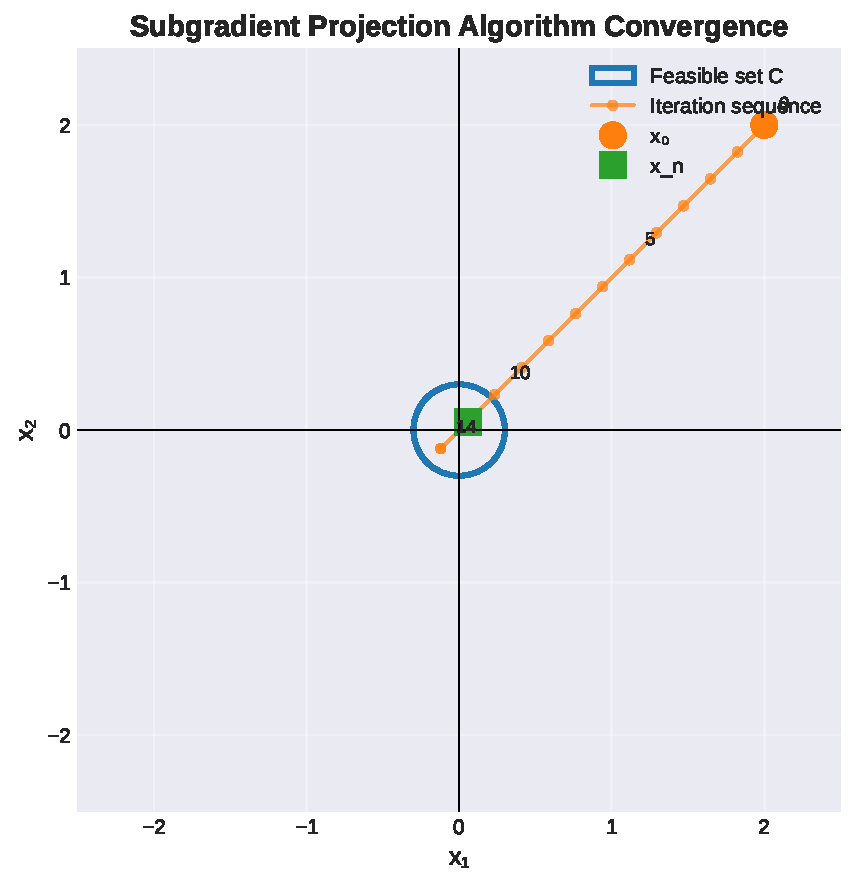
\includegraphics[width=\textwidth]{fig_algorithm_convergence.pdf}

        \column{0.5\textwidth}
        \begin{itemize}
            \item Iterates spiral inward toward feasible region

            \item Step size adapts based on constraint violation

            \item Projection ensures feasibility at each step

            \item Convergence guaranteed under mild conditions
        \end{itemize}
    \end{columns}
\end{frame}

\begin{frame}{Convergence Rates Comparison}
    \begin{columns}
        \column{0.5\textwidth}
        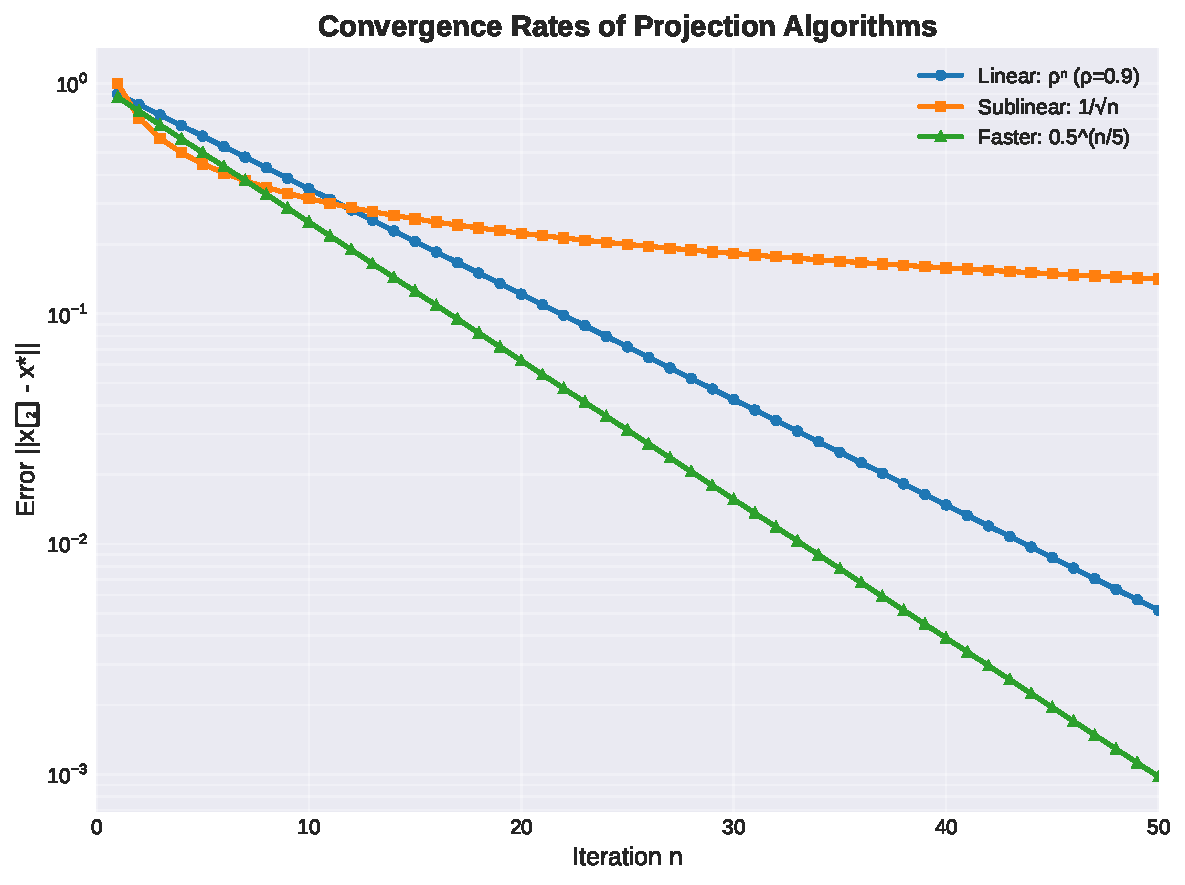
\includegraphics[width=\textwidth]{fig_convergence_rate.pdf}

        \column{0.5\textwidth}
        \begin{itemize}
            \item \textbf{Linear}: $\|e_n\| \sim \rho^n$ (fastest, $\rho < 1$)

            \item \textbf{Sublinear}: $\|e_n\| \sim 1/\sqrt{n}$ (slow but guaranteed)

            \item \textbf{Behavior}:
            \begin{itemize}
                \item Problem conditioning matters
                \item Smooth problems: fast
                \item Non-smooth: slower
                \item Degenerate: sublinear
            \end{itemize}

            \item \textbf{Practical}: Accelerated variants often needed
        \end{itemize}
    \end{columns}
\end{frame}

% ============================================================================
% SECTION 7: PYTHON EXAMPLES
% ============================================================================
\section{Python Implementation Examples}

\begin{frame}[fragile]{Basic Projection Implementation}

    \begin{lstlisting}
import numpy as np
from scipy.optimize import minimize

def proj_box(x, a, b):
    """Projection onto box [a,b]^n"""
    return np.clip(x, a, b)

def proj_ball(x, radius=1.0):
    """Projection onto Euclidean ball"""
    norm_x = np.linalg.norm(x)
    if norm_x <= radius:
        return x.copy()
    return (radius / norm_x) * x

def proj_halfspace(x, u, eta):
    """Projection onto {y : <y,u> <= eta}"""
    inner = np.dot(x, u)
    if inner <= eta:
        return x.copy()
    return x - (inner - eta) * u / np.dot(u, u)

# Test
x = np.array([2.0, 3.0])
print(f"Proj onto ball: {proj_ball(x, radius=2)}")
print(f"Proj onto box: {proj_box(x, a=0, b=2)}")
print(f"Proj onto HS: {proj_halfspace(x, u=np.ones(2), eta=1)}")
    \end{lstlisting}

\end{frame}

\begin{frame}[fragile]{Probability Simplex Projection}

    \begin{lstlisting}
def proj_simplex(x):
    """Project x onto probability simplex
    min ||y - x||^2 s.t. y >= 0, sum(y) = 1
    """
    n = len(x)
    # Sort x in descending order
    u = np.sort(x)[::-1]

    # Find rho: largest i such that u[i] > (sum(u[:i+1]) - 1) / (i+1)
    cssv = np.cumsum(u)
    rho = np.where(u > (cssv - 1) / np.arange(1, n+1))[0][-1]

    # Compute threshold
    theta = (cssv[rho] - 1) / (rho + 1)

    # Apply threshold and rectify
    y = np.maximum(x - theta, 0)
    return y

# Example: project outside simplex
x = np.array([2.0, 0.5, -1.0])
y = proj_simplex(x)
print(f"Original: {x}")
print(f"Projected: {y}")
print(f"Valid: sum={y.sum()}, nonneg={np.all(y >= 0)}")
    \end{lstlisting}

\end{frame}

\begin{frame}[fragile]{Alternating Projections Algorithm}

    \begin{lstlisting}
def alternating_projections(P1, P2, x0, max_iter=1000, tol=1e-6):
    """
    Alternating projections: x_{n+1} = P2(P1(x_n))
    Used for finding point in intersection of two sets
    """
    x = x0.copy()
    history = [np.linalg.norm(x)]

    for n in range(max_iter):
        x_prev = x.copy()
        x = P2(P1(x))  # Alternate between projections

        error = np.linalg.norm(x - x_prev)
        history.append(error)

        if error < tol:
            print(f"Converged in {n+1} iterations")
            return x, history

    print(f"Max iterations reached")
    return x, history

# Example: intersection of two balls
def proj_ball1(x):
    return proj_ball(x - np.array([0.5, 0]), radius=1.0) + np.array([0.5, 0])

def proj_ball2(x):
    return proj_ball(x - np.array([-0.5, 0]), radius=1.0) + np.array([-0.5, 0])

x0 = np.array([1.0, 1.0])
x_sol, hist = alternating_projections(proj_ball1, proj_ball2, x0)
print(f"Solution: {x_sol}")
    \end{lstlisting}

\end{frame}

\begin{frame}[fragile]{Proximal Operator and Projection Connection}

    \begin{lstlisting}
def prox_convex_fn(f, grad_f, x, gamma=0.1, max_iter=20):
    """Compute prox_gamma_f(x) using gradient descent"""
    y = x.copy()
    for _ in range(max_iter):
        y = y - gamma * (grad_f(y) + 2/gamma * (y - x))
    return y

def proj_epi(f, grad_f, x, eta):
    """Project onto epigraph of f: epi f = {(x,t) : f(x) <= t}"""
    # If already in epigraph, stay put
    if f(x) <= eta:
        return x, eta

    # Otherwise, minimize distance to epigraph
    # This involves solving a subdifferential inclusion
    x_proj = prox_convex_fn(f, grad_f, x)
    f_proj = f(x_proj)

    if f_proj < eta:
        # Project onto boundary
        return x_proj, f_proj
    else:
        # On the boundary
        return x_proj, eta

# Example: f(x) = ||x||^2
f = lambda x: np.sum(x**2)
grad_f = lambda x: 2*x

x = np.array([2.0, 3.0])
x_proj, eta_proj = proj_epi(f, grad_f, x, eta=5.0)
print(f"Original: ({x}, inf)")
print(f"Projected onto epi f: ({x_proj}, {eta_proj})")
    \end{lstlisting}

\end{frame}

% ============================================================================
% SECTION 8: APPLICATIONS
% ============================================================================
\section{Applications and Extensions}

\begin{frame}{Key Applications}

    \begin{enumerate}
        \item[\textbf{1}] \textbf{Convex Feasibility}
        \begin{itemize}
            \item Find point in $C_1 \cap C_2 \cap \cdots \cap C_m$
            \item Use alternating projections: $x_{n+1} = P_{C_{i_n}}(x_n)$
            \item Guarantees weak convergence under standard conditions
        \end{itemize}

        \vspace{0.3cm}

        \item[\textbf{2}] \textbf{Constrained Optimization}
        \begin{itemize}
            \item Minimize $f(x)$ subject to $x \in C$
            \item Combine gradient/subgradient with projection
            \item Example: Projected gradient descent $x_{n+1} = P_C(x_n - \gamma \nabla f(x_n))$
        \end{itemize}

        \vspace{0.3cm}

        \item[\textbf{3}] \textbf{Image Processing}
        \begin{itemize}
            \item Denoise via projection onto convex set of ``good'' images
            \item Convex constraints: total variation, sparsity, etc.
            \item Fast iterative methods essential
        \end{itemize}

        \vspace{0.3cm}

        \item[\textbf{4}] \textbf{Signal Recovery}
        \begin{itemize}
            \item Compressed sensing: recover sparse signal from few measurements
            \item Projection onto $\ell_1$ ball or simplex
            \item Efficient algorithms critical
        \end{itemize}
    \end{enumerate}

\end{frame}

\begin{frame}{Connection to Proximal Methods}

    \textbf{Proximal Operator and Projection}:\\
    The \textit{proximal operator} is a generalization of projections:
    $$\text{prox}_{\gamma f}(x) = \arg\min_y \left\{ f(y) + \frac{1}{2\gamma}\|y - x\|^2 \right\}$$

    \vspace{0.3cm}

    When $f = \iota_C$ (indicator function of $C$):
    $$\text{prox}_{\gamma \iota_C}(x) = P_C(x)$$

    \vspace{0.5cm}

    \textbf{Splitting Methods}:\\
    For $f = g + h$:
    $$\text{Forward-Backward Splitting}: x_{n+1} = \text{prox}_{\gamma h}(x_n - \gamma \nabla g(x_n))$$

    When $g = 0$, reduces to fixed point of proximal operator.\\
    When $h = \iota_C$, becomes projected gradient method!

\end{frame}

% ============================================================================
% SECTION 9: SUMMARY
% ============================================================================
\section{Summary \& Key Takeaways}

\begin{frame}{Main Results Summary}

    \begin{enumerate}
        \item[\textbf{Existence \& Uniqueness}]
        Projections onto nonempty closed convex sets are unique and well-defined.

        \vspace{0.2cm}

        \item[\textbf{Characterization}]
        Via variational inequality: $\langle x - P_C(x) \mid y - P_C(x) \rangle \leq 0$ for all $y \in C$.

        \vspace{0.2cm}

        \item[\textbf{Nonexpansiveness}]
        Projections are \textit{firmly nonexpansive} operators (stronger property).

        \vspace{0.2cm}

        \item[\textbf{Special Cases}]
        Explicit formulas for half-spaces, simplices, ellipsoids, boxes, etc.

        \vspace{0.2cm}

        \item[\textbf{Algorithms}]
        Subgradient projection methods converge weakly to constrained minimizers.

        \vspace{0.2cm}

        \item[\textbf{Computational}]
        Many projections have efficient algorithms ($O(n)$ or $O(n\log n)$).

        \vspace{0.2cm}

        \item[\textbf{Connections}]
        Proximal operators generalize projections; splitting methods unify many algorithms.
    \end{enumerate}

\end{frame}

\begin{frame}{Important Insights}

    \begin{itemize}
        \item \textbf{Projection is orthogonal}: The residual $x - P_C(x)$ is perpendicular to all directions into $C$.

        \vspace{0.3cm}

        \item \textbf{Contraction property}: Projections reduce distances between points (firm nonexpansiveness).

        \vspace{0.3cm}

        \item \textbf{Versatility}: Same operation (projection) used in optimization, feasibility, and fixed-point problems.

        \vspace{0.3cm}

        \item \textbf{Structure matters}: Different set structures (half-space, simplex, box) have different computational costs.

        \vspace{0.3cm}

        \item \textbf{Weak convergence}: Most projection algorithms converge weakly; strong convergence requires additional structure.

        \vspace{0.3cm}

        \item \textbf{Generalization}: Proximal operators and splitting methods extend projection ideas to broader optimization problems.
    \end{itemize}

\end{frame}

\begin{frame}{Further Reading}

    \begin{itemize}
        \item \textbf{Bauschke \& Combettes (2017)}: ``Convex Analysis and Monotone Operator Theory in Hilbert Spaces''
        \begin{itemize}
            \item Chapters 24--30 cover projections, proximal methods, and splitting algorithms
            \item Comprehensive treatment with many examples
        \end{itemize}

        \vspace{0.3cm}

        \item \textbf{Boyd \& Parikh (2011)}: ``Proximal Algorithms''
        \begin{itemize}
            \item Practical implementation guidance
            \item Applications to machine learning and statistics
        \end{itemize}

        \vspace{0.3cm}

        \item \textbf{Nesterov (2018)}: ``Lectures on Convex Optimization''
        \begin{itemize}
            \item Convergence analysis with complexity bounds
            \item Accelerated methods
        \end{itemize}

        \vspace{0.3cm}

        \item \textbf{Recent Applications}:
        \begin{itemize}
            \item Machine learning: federated learning, distributed optimization
            \item Signal processing: compressed sensing, sparse recovery
            \item Computer vision: image denoising, inpainting
        \end{itemize}
    \end{itemize}

\end{frame}

\end{document}
